\section{Dataset}

%%%%%%%%%%%%%%%%%%%%%%%%%%%%%%%%%%%%%%%%%%%%%%%%%%%%%%%
% Binary Data Stats
%%%%%%%%%%%%%%%%%%%%%%%%%%%%%%%%%%%%%%%%%%%%
\begin{table}[t]
\centering
\resizebox{\columnwidth}{!}{%
\begin{tabular}{lrrrr}
\hline
\multirow{2}{*}{\textbf{Metric}} & \multicolumn{2}{c}{\textbf{Train}} & \multirow{2}{*}{\textbf{Validation}} & \multirow{2}{*}{\textbf{Test}} \\
\cmidrule{2-3}
& \textbf{multi} & \textbf{single} &         &         \\ \hline
\multicolumn{5}{c}{\textbf{SCI}}                                             \\ \hline
\#Documents      & 35,942          & 20,712           & 2,960    & 5,919    \\
Avg \#words  & 2,738        & 2,734         & 2,638 & 2,731 \\
Acceptance(\%) & 59.37          & 50.79           & 50.74   & 50.87   \\ \hline
\multicolumn{5}{c}{\textbf{SCI + HCs}}                      \\
\hline
\#Documents       & 4,84,725         & 2,83,457          & 40,495   & 80,988   \\
Avg \#words  & 2,168        & 2,115         & 2,096 & 2,107 \\
Acceptance(\%) & 55.75          & 51.94           & 48.22   & 48.25   \\  \hline
\multicolumn{5}{c}{\textbf{SCI + HCs + Tribunals}} \\
\hline
\#Documents       & 6,48,356         & 3,68,639        & 52,663   & 1,05,326  \\
Avg \#words  & 2,081        & 1,999         & 2,003 & 1,989 \\
Acceptance(\%) & 58.27          & 49.48           & 49.49   & 49.36   \\ \hline
\multicolumn{5}{c}{\textbf{SCI + HCs + Tribunals + Daily Orders and District Courts}}    \\
\hline
\#Documents       & 7,02,945         & 4,01,412         & 57,345   & 1,14,690  \\
Avg \#words  & 2,061        & 1,985         & 1,987 & 1,976 \\
Acceptance(\%) & 57.98          & 49.30           & 49.34   & 49.04  
\\ \hline
\end{tabular}%
}
\caption{Data statistics across different courts for evaluating model performance on binary classification.}
\label{tab:binary-stats}
\end{table}

%%%%%%%%%%%%%%%%%%%%%%%%%%%%%%%%%%%%%%%%%%%
% Ternary Data Stats
%%%%%%%%%%%%%%%%%%%%%%%%%%%%%%%%%%%%%%%%%%%
\begin{table}[t]
\centering
\resizebox{\columnwidth}{!}{%
\begin{tabular}{lrrr}
\hline
\textbf{Metric}  & \textbf{Train}   & \textbf{Validation}   & \textbf{Test}  
\\ \hline
\multicolumn{4}{c}{\textbf{SCI}}     
\\ \hline
\#Documents               & 26,823            & 3,833                 & 7,665           \\
Avg \#words               & 2,777          & 2,779               & 2,783        \\
Clear acceptance(\%)      & 41.95            & 41.22                 & 41.44          \\
Partial acceptance (\%)   & 17.19            & 18.03                 & 17.59          \\ \hline
\multicolumn{4}{c}{\textbf{SCI + HCs}}                      \\
\hline
\#Documents               & 3,40,972           & 48,711                 & 97,421          \\
Avg \#words               & 2,173          & 2,166               & 2,180        \\ 
Clear acceptance(\%)      & 54.31            & 54.46                 & 54.56          \\
Partial acceptance (\%)   & 1.38             & 1.29                  & 1.34           \\ \hline
\multicolumn{4}{c}{\textbf{SCI + HCs + Tribunals}}                                                            \\
\hline
\#Documents               & 4,55,514           & 65,074                 & 1,30,147         \\
Avg \#words               & 2,085          & 2,082               & 2,089        \\
Clear acceptance(\%)      & 57.23            & 57.55                 & 57.10          \\
Partial acceptance (\%)   & 1.03             & 0.96                  & 1.03           \\ \hline
\multicolumn{4}{c}{\textbf{SCI + HCs + Tribunals + Daily Orders and District Courts}}    \\
\hline
\#Documents               & 4,93,726           & 70,533                 & 1,41,065         \\
Avg \#words               & 2,061          & 2,068               & 2,081        \\
Clear acceptance(\%)      & 57.02            & 56.83                 & 57.14          \\
Partial acceptance (\%)   & 0.94             & 0.97                  & 0.95   \\ \hline       
\end{tabular}%
}
\caption{Data statistics across different courts for evaluating model performance on ternary classification.}
\label{tab:ternary-stats}
\end{table}
%%%%%%%%%%%%%%%%%%%%%%%%%%%%%%%%%%%%%%%%%%%%%

We introduce the dataset \textbf{\texttt{\named}}, which is the largest and most diverse corpus of Indian legal cases ever compiled, covering judgments from the Supreme Court, High Courts, Tribunal courts, District courts, and Daily orders. This comprehensive dataset offers unparalleled diversity and coverage, addressing existing gaps and providing a rich foundation for advanced legal AI research.

\subsection{Dataset Compilation}

The dataset compilation process involved gathering a corpus of 22,82,137 Indian court case proceedings up to April 2024. We utilized the IndianKanoon website\footnote{\url{https://indiankanoon.org/}}, a well-known legal search engine, to collect these documents. This source is widely recognized for its comprehensive database of Indian legal documents, making it an invaluable resource for our dataset.

\subsection{Data Statistics} 

The \texttt{\named} dataset exhibits extensive data statistics, vital for understanding the dataset's scope and characteristics. The overall dataset is divided into `multi' and `single' categories based on the nature of the decisions. Table~\ref{tab:binary-stats} and Table~\ref{tab:ternary-stats} provide detailed statistics, including the number of documents, the average number of tokens, and the distribution of clear and partial acceptance decisions across the dataset. This dataset is also analyzed on a court-wise basis, providing insights into the unique characteristics of cases from different courts.
Figure~\ref{fig:court-distribution} in the Appendix shows the distribution of cases in different courts in percentage. This breakdown helps in understanding the diversity within the dataset and the varying complexities associated with different court levels.


% %%%%%%%%%%%%%%%%%%%%%%%%%%%%%%%%%%%%%%%%%%%%%
% \begin{figure}[t]
%     \centering
%     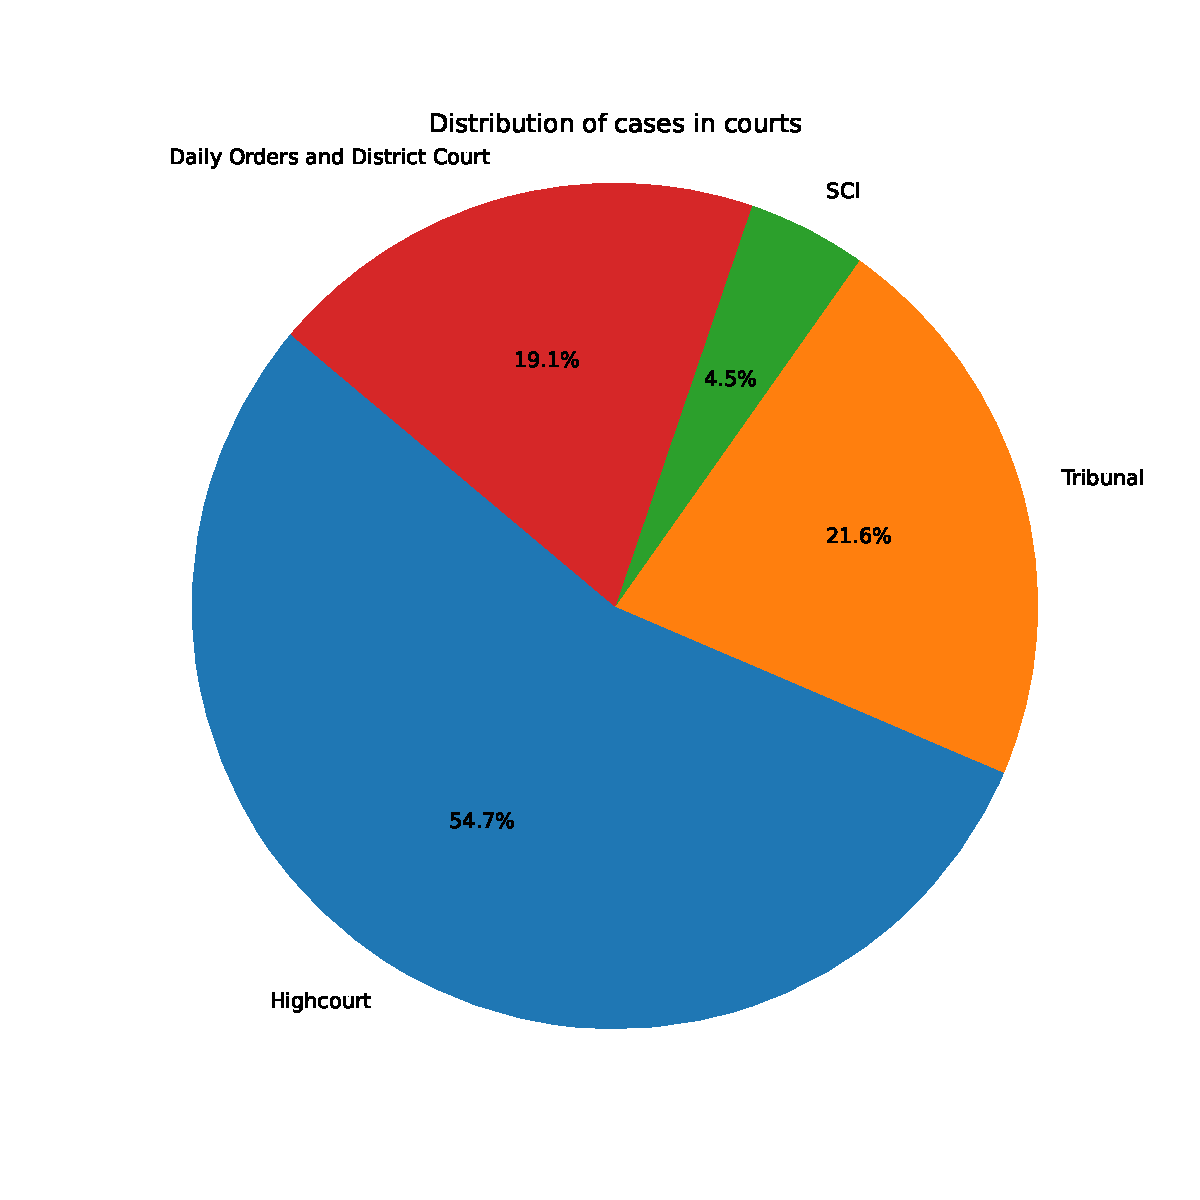
\includegraphics[width=\columnwidth]{figures/pre-processed-all-courts-pie-chart_cropped.pdf}
%     \caption{Distribution of cases in different courts (percentage).}
%     \label{fig:court-distribution}
% \end{figure}
% %%%%%%%%%%%%%%%%%%%%%%%%%%%%%%%%%%%%

\subsubsection{Injecting Legal Knowledge}
To address the deficiency of legal knowledge in the base LLaMa model, we employed a \emph{continued pretraining (CPT)} approach using a comprehensive Indian legal corpus. Due to resource constraints, we used a subset of the full \texttt{\named} dataset for this pretraining phase. This subset includes preprocessed data comprising 38,321 cases from the Supreme Court of India (SCI) and a randomly selected 1,00,000 cases from various High Courts. These choices were made to balance computational feasibility and the inclusion of diverse and representative legal cases. This extensive yet manageable training corpus was essential for embedding domain-specific legal knowledge into the model. Additionally, the validation dataset consisted of 12,239 documents sourced from both SCI and High Courts, ensuring that the model was rigorously tested and fine-tuned for the nuances of the Indian legal system. By focusing on a strategically chosen subset, we aimed to maximize the impact of the training within the available computational resources. This approach enhances the model's understanding and applicability within the Indian legal framework, thereby improving its predictive capabilities and relevance in legal tasks.


\subsubsection{Learning Reasoning Skills}
To equip the model with the necessary reasoning capabilities for solving prediction and explanation problems, we conducted \emph{supervised fine-tuning (SFT)} using selected data from downstream tasks on the PredEx training dataset \cite{nigam2024legaljudgmentreimaginedpredex}, which consists of 12,178 cases accompanied by corresponding case decisions and explanations annotated by legal experts. By performing SFT on this dataset, we aimed to enhance its reasoning skills and ability to comprehend and apply legal principles effectively. This targeted fine-tuning approach helps bridge the gap between the model's general knowledge and the specific requirements of legal reasoning tasks, ultimately improving its performance in real-world legal scenarios.

\subsubsection{Prediction Task}

For prediction, we split the \texttt{\named} single dataset into training, validation, and test sets in the ratio 70:10:20. A key component of our research involved comparing the performance of models trained on \texttt{\named} with those trained on the ILDC 2021 \cite{malik-etal-2021-ildc} test dataset. This comparison is crucial for benchmarking our models and understanding their efficacy compared to established datasets in the field. By testing against ILDC 2021, we aim to evaluate the improvements in prediction accuracy and model robustness that \texttt{\named} offers, showcasing its contribution to the evolving landscape of legal AI in India.
We also tested the model performance on temporal data, assessing its effectiveness on future or unseen data from January 2020 to April 2024 to ensure robustness and generalization capabilities over time, as detailed in Table \ref{tab:temporal-test-cases}.

%%%%%%%%%%%%%%%%%%%%%%%%%%%%%%%%%%%%%%%%%%%%
% Temporal Data Stats
%%%%%%%%%%%%%%%%%%%%%%%%%%%%%%%%%%%%%%%%%%%%

\begin{table}[t]
\centering
\resizebox{\columnwidth}{!}{%
\begin{tabular}{lrrrr}
\hline
\textbf{Metric}  &
  \textbf{SCI} &
  \textbf{HCs} &
  \textbf{Tribunals} &
  \textbf{\begin{tabular}[c]{@{}c@{}}Daily Orders and\\ District Courts\end{tabular}} \\ \hline
\textbf{\#Documents}      & 1,812    & 29,216   & 19,034   & 17,002   \\ 
\textbf{Avg \#words}  & 4,470 & 2,671 & 2,927 & 1,306 \\ 
\textbf{Acceptance (\%)} & 67.77   & 53.18   & 47.42   & 62.40   \\ \hline
\end{tabular}%
}
\caption{Statistics of temporal test data (January 2020 -- April 2024) across different courts for evaluation.}
\label{tab:temporal-test-cases}
\end{table}
%%%%%%%%%%%%%%%%%%%%%%%%%%%%%%%%%%%%%%%%%%%%%

\subsubsection{Prediction with Explanation Task}
For this task, we used the PredEx 2024 test dataset \cite{nigam2024legaljudgmentreimaginedpredex}, which includes 3,044 balanced cases. The balanced nature of the test set is particularly important for maintaining the validity of our experiments and ensuring the reliability and generalizability of our model's performance.

% Overall, \texttt{\named} stands as a pioneering dataset in the realm of LJP, offering unprecedented depth, diversity, and scope for exploring legal AI in the Indian context. \ab{this paragraph seems unnecessary}
